\section{Problem 1 – Linear Algebra}

\paragraph{Question 1}
Let $x$ be an eigenvector with corresponding eigenvalue $\lambda$: $Ax = \lambda x$.
Let $\mu \in \mathbb{R}$. 
\begin{equation*}
    (A + \mu I)x = Ax + \mu x = \lambda x + \mu x = (\lambda + \mu)x
\end{equation*}
So $x$ is an eigenvector of $(A + \mu I)$ with corresponding eigenvalue of $\lambda + \mu$.


\paragraph{Question 2}
Let $v \in \mathbb{R^N}$ be a unit vector which maximizes $v^T A v$.
Because $A$ is real and symmetric, then it can be diagonalized $A = Q^T \Lambda Q$, where $Q$ is orthogonal matrix, which columns form orthogonal basis.
In following equation, let's substitute $y = Qv$:
\begin{align*}
    v^T A v &= v^T Q^T \Lambda Q v = y^T \Lambda y \\
            &= \sum_{i=1}^{N}\lambda_i y_i^2\\
            &\leq \: \sum_{i=1}^{N} \lambda_{max}(A) \: y_i^2
              = \lambda_{max}(A) \: \sum_{i=1}^{N} y_i^2\\
            &= \lambda_{max}(A) \: y^T y = \lambda_{max}(A) \: v^T Q^T Q v\\
            &= \lambda_{max}(A)
\end{align*}
On the other hand, let $x_{max}$ be eigenvector corresponding to $\lambda_{max}(A)$.
Because $v$ maximizes $v^T A v$, then:
\begin{equation*}
    v^T A v \geq x_{max}^T (A x_{max} ) = x_{max}^T  x_{max} \: \lambda_{max}(A)  = \lambda_{max}(A)
\end{equation*}
Here we got:
\begin{equation*}
    \lambda_{max}(A) \leq v^T A v \leq \lambda_{max}(A)
\end{equation*}
For vector $v$ which maximizes $v^T A v$.
Hence,
\begin{equation*}
    \lambda_{max}(A) = \max \{v^T A v | v\in\mathbb{R}^N, v^T v = 1\}
\end{equation*}
and the maximum is reached for eigenvector $x_{max}$.

\paragraph{Question 2}
 Let $v\in\mathbb{R}^N$.
From question (2) we know that $v^T A v\leq \lambda_{max}(A) v^T v$ for arbitrary $v$: look at second to the last line of Q2 calculations.
Now if we know that fact, we get the inequality trivially:

\begin{align*}
    v^T(\lambda_{max}(A) I - A) v 
        = \lambda_{max}(A) v^T v - v^T A v
        \geq 0
\end{align*}


\paragraph{Question 3}
Since $A, B$ are symmetric and real, then $A = Q^T\Lambda_A Q$ and $B = P^T\Lambda_B P$ for some orthogonal $Q$~and~$P$.
From what we obtained in (Q2): let $w$ be a~unit vector which maximizes $w^T(A+B)w$.
Then:
\begin{align*}
    \Lambda_{max}(A+B) &= w^T(A+B)w \\
                        &= w^T A w + w^T B w \\
                        &= w^T Q^T \Lambda_A Q w + w^T P^T \Lambda_B P w = (*)
\end{align*} 
Substitute $y = Qw$ and $z = Pw$. Of course $y^T y = z^T z = 1$, because $y^T y = w^TQ^TQw = w^T w = 1$ (the same for $z$).
Combining this and our knowledge form previous questions:
\begin{align*}
    (*) &= y^T \Lambda_A y + z^T \Lambda_B z \\
            &\leq \lambda_{max}(A) \: y^T y + \lambda_{max}(B) \: z^T z \\
            &= \lambda_{max}(A) + \lambda_{max}(B)
\end{align*}


\section{Problem 2 – Automata theory}
\paragraph{Question 1}
\emph{This one was also solved in \textbf{Automata Theory, Languages and computation 3rd ed}, 2.2.4, Example 2.4}
\begin{figure}[!h]
    \centering
    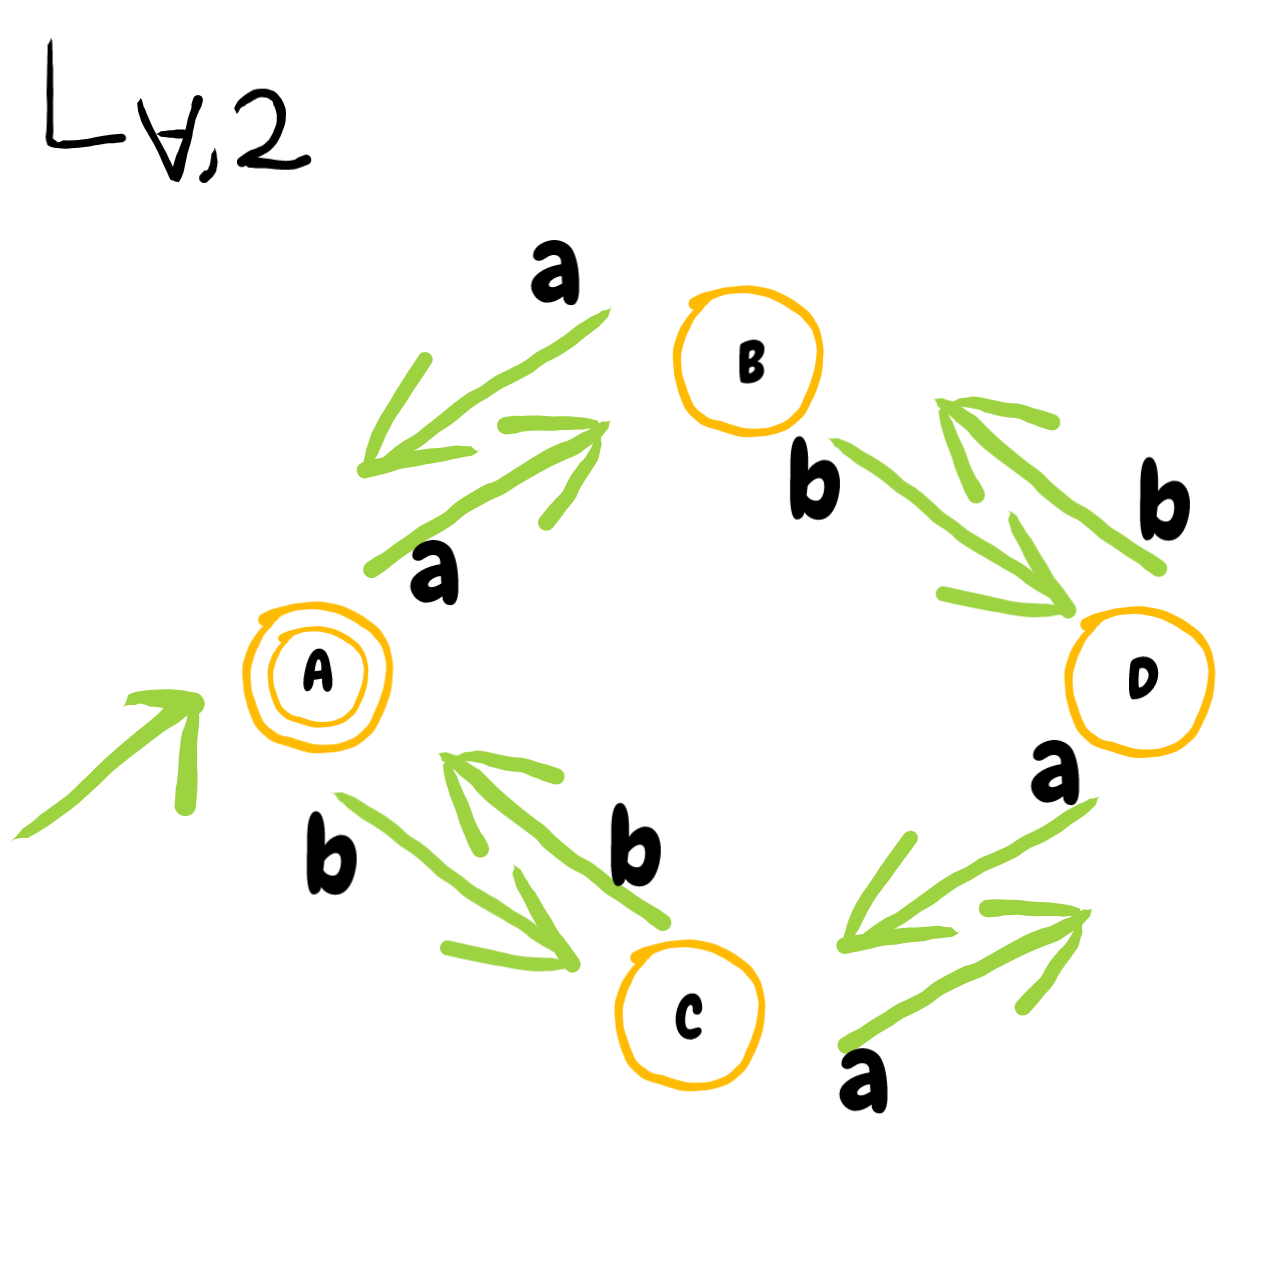
\includegraphics[scale=0.3]{data/2018-W-2-1.png}
    \caption{Question 1.}
\end{figure}



Explanation:
\begin{itemize}
    \item A – "number of $a$'s is \textbf{even}, number of $b$'s is \textbf{even}"
    \item B – "number of $a$'s is \textbf{odd}, number of $b$'s is \textbf{even}"
    \item C – "number of $a$'s is \textbf{even}, number of $b$'s is \textbf{odd}"
    \item D – "number of $a$'s is \textbf{odd}, number of $b$'s is \textbf{odd}"
\end{itemize}


\paragraph{Question 2}
Begin with an $\epsilon$-NFA as depiced in Fig. \ref{fig:w1822a}.
It "guesses" which letter appears even number of times.
To make it $\epsilon$-free, we either follow him: \url{https://youtu.be/sq-dLKAd6bo?t=1714} or consider the followig:
starting from start state, how far, i.e. which states can we reach on letter $a$?
There are $3$ such states.
We simply draw an edge to those states.
Do the same for $b,c$. 
The final answer is on Fig. \ref{fig:w1822b}
\begin{figure}[!h]
    \centering
    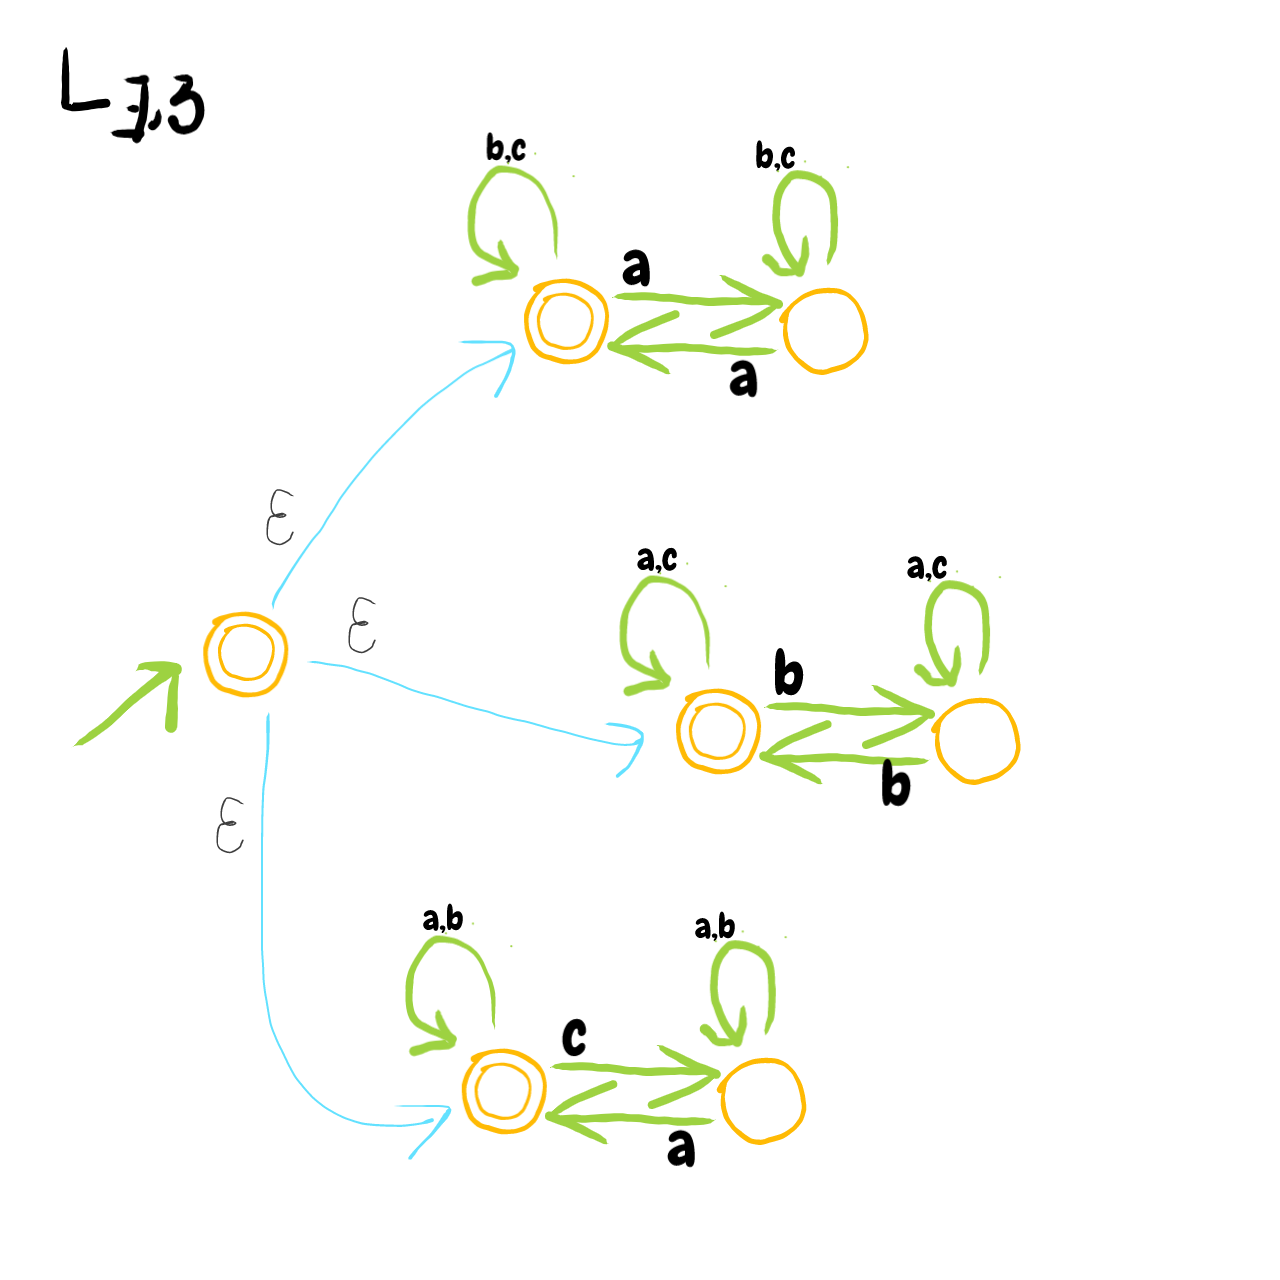
\includegraphics[scale=0.3]{data/2018-W-2-2a.png}
    \caption{Question 2.  $\epsilon$-NFA.}
    \label{fig:w1822a}
\end{figure}
\begin{figure}[!h]
    \centering
    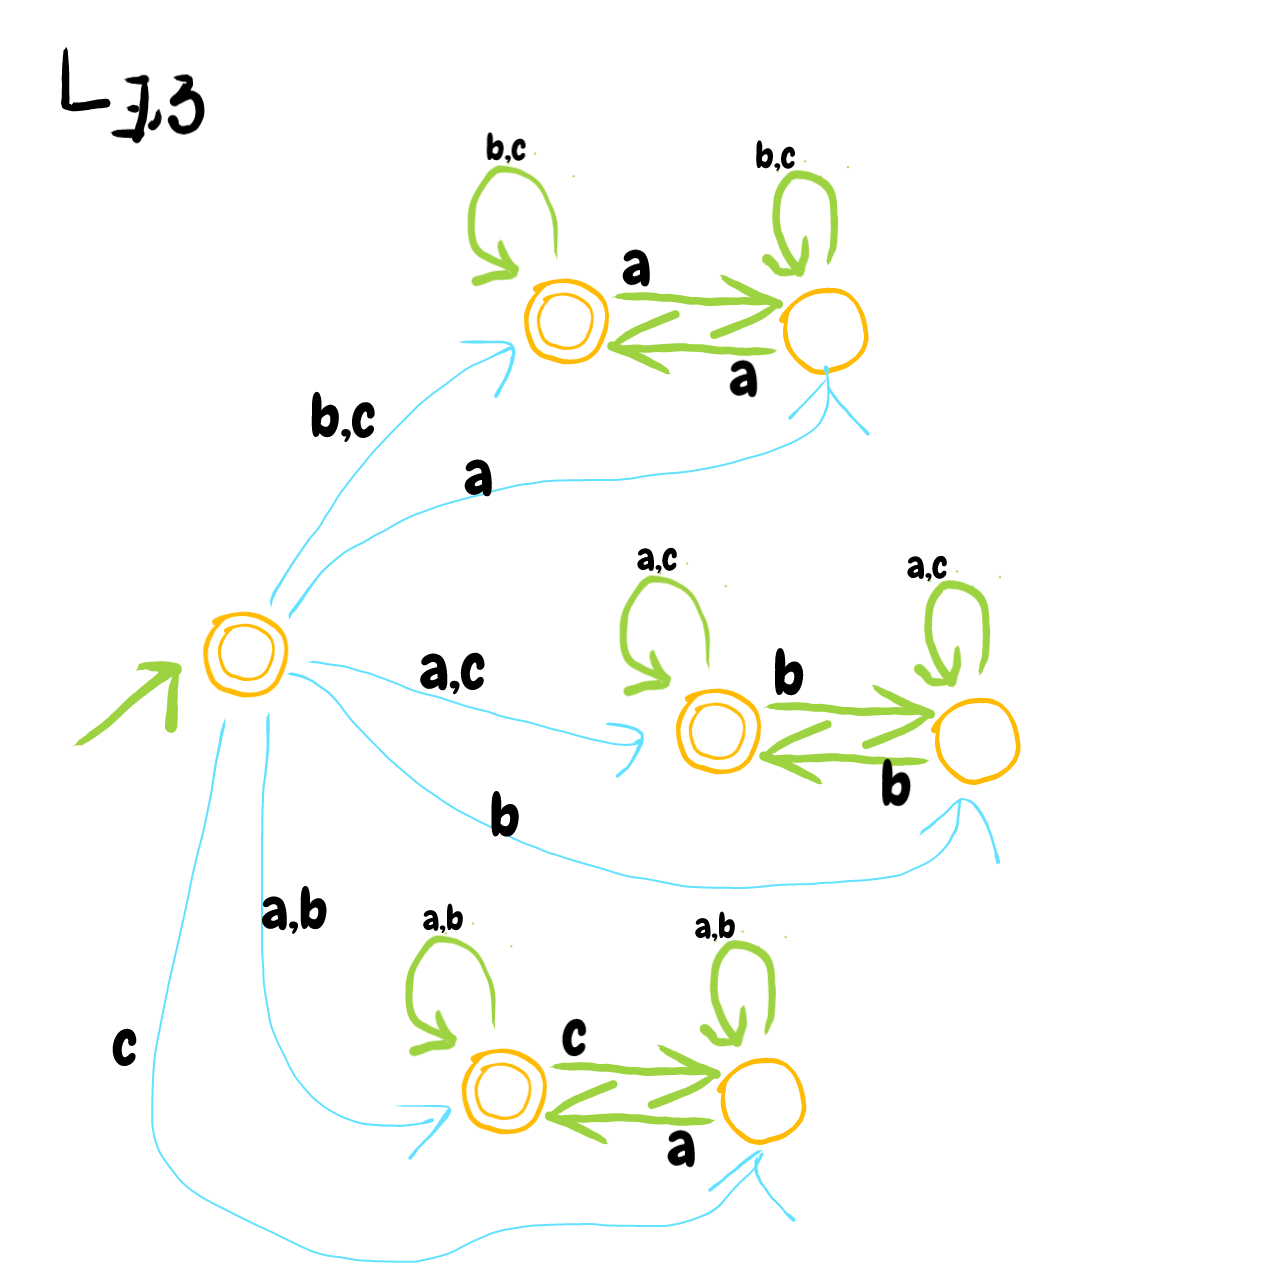
\includegraphics[scale=0.3]{data/2018-W-2-2b.png}
    \caption{Question 2. $\epsilon$-free NFA. We followed former $\epsilon$-transitions and added new edges (in blue). Thanks Taku!}
    \label{fig:w1822b}
\end{figure}




\paragraph{Question 3}
\emph{Prove that, for every $n\geq 1$, every \textbf{deterministic} finite state automaton that accepts $L_{\exists ,n}$ has at least $2^n$ states.}

\emph{First, I'll show that there is a DFA with $2^n$ states.}
We can encode states of DFA $L_{\exists ,n}$ as a binary string $B = (b_n, b_{n-1}, \cdots, b_2, b_1)$ of length $n$, where $b_i = 1$ iff numbers of $a_i$'s is odd in so-far read sequence, else $0$.
A state is accepting if its binary representation has at least one zero.
There are $2^n$ such strings.

\emph{Now, I'll show that there is no DFA with less than $2^n$ states.}
If the DFA had fewer than $2^n$ states, then there would be some state $q$ such that the DFA can be in state $q$ after reading two different sequences of length $n$, say $a = a_1a_2\cdots a_n$ and $b = b_1b_2\cdots b_n$.
If the sequences were of \emph{different parity}, i.e. one of the sequences had a letter which appears even number of times, and the other sequence hadn't, then $q$ would be both accepting and nonaccepting state.
If the sequences were of the same parity, then we could append some sequence $c_1\cdots c_m \in \Sigma^*$ to $a$ and $b$ such that $a_1a_2\cdots a_n c_1\cdots c_m$ and $b_1b_2\cdots b_n c_1\cdots c_m$ have different parity.
Consider state $p$ that the DFA enters after reading $c_1\cdots c_m$. 
Then $p$ must be both accepting and nonaccepting, since either of
$a_1a_2\cdots a_n c_1\cdots c_m$ and $b_1b_2\cdots b_n c_1\cdots c_m$ is accepted and the other isn't.

This problem could be also one-lined using \textit{Myhill-Nerode theorem}.
The only one difficulty here is to define $2^n$ equivalent classes.
Try fiddling with binary strings.



\paragraph{Question 4}
\emph{Prove that, for every $n\geq 1$, every \textbf{non-deterministic} finite state automaton (without $\epsilon$-transitions) that accepts $L_{\forall ,n}$ has at least $2^n$ states.}
Begin with constructing DFA $A$ accepting $L_{\forall ,n}$ the same way as in Q3 – except that $A$ has only one accepting state, a string of all $0$'s.
Obviously this DFA is also a~NFA.
The equivalent NFA simply cannot \textit{guess} parity of some letters: it has to remember information of parity of each letter.
As shown in Q3, every letter requires $2$ bits, so minimum of $2^n$ states are required.

\emph{s e n d h e l p}




\section{Problem 3 – Union-Find}
\emph{See chapter $21$ of Cormen (3rd edition) for more.}

We have set of $2^N$ elements. 
\emph{MERGE}($A, B$) changes $A$'s root's pointer so that it points root of $B$.

\paragraph{Question 1}
$2^N-1$ merge operations are required to merge all the subsets.

\paragraph{Question 2}
Minimum tree height: $1$ – one root with $2^N - 1$ leafs. 
How to: Fix root $r$ and perform \emph{MERGE}($v, r$) for every other element $v \neq r$.

\paragraph{Question 3}
Maximum tree height: $2^N -1$.
How to: start with a tree consisting of one element.
While merging the tree and a node, make the tree point the node.
In pseudo-code: 
\begin{verbatim}
for i in range(1, 2**N):
    merge(v[i-1], v[i])
\end{verbatim}


\paragraph{Question 4}
New MERGE(A, B): change pointer of the root node of subset with smaller height so that it points to root node of the other subset. 
This technique is called \emph{merge (union) by rank} (rank - upper bound on the height of the node).
How to get a tree with maximum height?
The observation is, merging trees having the same height will result in a taller tree.
If $A$ and $B$ have height of $h$, then merged tree is of height $h+1$.

Suppose we had a maximum-height tree with $2^N$ nodes.
It must have been obtained by merging of two maximum-height trees with $2^{N-1}$ nodes.
\begin{equation*}
    H(2^N) = 1 + H(2^{N-1}) = N
\end{equation*}


\paragraph{Question 4}
During execution of FIND, we make every node on the find-path point directly to the root.
This technique is called \emph{path compression}.

In details, first we find a path from a node its root. 
Then, we go through the path again and change pointers of nodes on the path.
Original FIND was linear in length of the path.
Now we scan the path twice, which still yields linear time.



\section{Problem 4 –  Synchronization}

\paragraph{Question 1}
Its $1$ and $2$.
On a sequential execution we get $2$.
We can get $1$ when one process loads a value before another process stores it.

\paragraph{Question 2}
Test-and-set writes $1$ to memory and returns previously stored value.

\begin{verbatim}
int TestAndSet(int *a) {
    int b;
    b = *a;
    *a = 1;
    return b;
}
\end{verbatim}


\paragraph{Question 3}
Swap:
\begin{verbatim}
void Swap(int *a, int *b) {
    int tmp = *a;
    *a = *b;
    *b = tmp;
}
\end{verbatim}
Answer:
\begin{verbatim}
int key = 1;
while (key == 1)
    Swap(&key, &lock);
x = x + 1;
lock = 0;
\end{verbatim}

